\chapter{Experimental Protocol}\label{Chapter:5}

The following chapter the design aspects introduced in previous chapters (\ref{ch:2},\ref{ch:3},\ref{Chapter:4}) are brought together and find their practical application. The goal is to produce measurable performance results  by applying of  preprocessing methods and statistical algorithms.

The general pattern that the experiment chapter is followed is partially inclined to the CRISP-DM process (see figure: \ref{fig:crisp-dm}) and contain three sub-processes: \textit{DataPreparation, Modelling, Evaluation}. Each of them contains techniques previously described in this Thesis. 

\begin{figure}[h!]
    \centering
    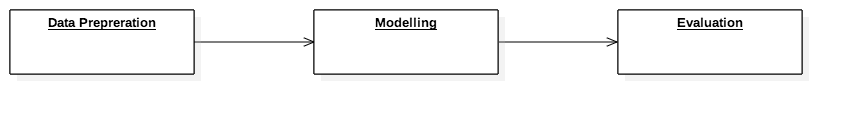
\includegraphics[scale=0.5]{Graphics/DeploymentDiagram1.png}
    \caption{General experiment pattern} %footnote?
    \label{fig:dep-dia}
\end{figure}

An experiment is defined as an process that follow the general experiment pattern (see figure: \ref{fig:dep-dia}), where the particular methods (see tables: \ref{tab:data-pred-methods}, \ref{tab:machine-learn-tech}, \ref{tab:res-ev}) and their parameters can vary.

This chapter is structured in two sections: First, the initial techniques and settings are given in chapter \ref{ch:5:ES}, then the results are presented in chapter \ref{Chapter:5:Results}. 


\section{Experiment Settintg (plan)} \label{ch:5:ES}

\textbf{Dataset description:}

The initial data set has \(95.951\) instances on \(1804\) features\footnote{A detailed overview of underlying data can be found in Chapter \ref{Ch:2:FeatureDesc}}. 
For all experiments, that are using algorithms based on positive and unlabeled data (One-Class SVM, PUL, SVM Ensemble), the data is divided into training, validation and test sets \((60\%/30\%/10\%)\).  All instances that are labeled as fraud \((744)\) are a member of the test set since the algorithms are utilized to treat unlabeled and  positively labeled data. 

All classification tasks are using 10-fold cross-validation. 


\begin{table}[ht!]
\centering
\setlength\tabcolsep{4pt}
\begin{minipage}{0.30\textwidth}
\centering
%\tablewidth=\textwidth
 \begin{tabular}{|l|l|}\hline
  Name&Reference\\ \hline
 Removing Corrupted Examples  & \ref{Ch:2:RCD} \\ \hline
        Categorical to Numeric Transform. & \ref{Ch:2:CTNT} \\
     \hline 
      Missing Value Imputation & \ref{Ch:2:MVI} \\
     \hline 
     
     Removing Zero- and Near-Zero Variance Features & \ref{Ch:2:RNZVF} \\
     \hline 

     Principle Component Analysis (PCA) & \ref{Ch:2:PCA} \\
     \hline 
        \end{tabular}
\caption{Data Preparation Methods.}
\label{tab:data-pred-methods} 
\end{minipage}%
\hfill
\begin{minipage}{0.24\textwidth}
\centering
 \begin{tabular}{|l|l|}\hline
         SVM & \ref{Chapter:SVM}\\
        \hline
        Two-Class SVM & \ref{Chapter:SVM} \\
        \hline
        One-Class SVM & \ref{Chapter:OC-SVM} \\
        \hline
        PU-Learning &  \ref{Chapter:PUL} \\
        \hline
        Ensemble SVM &  \ref{Chapter:Ensemble} \\
        \hline
        
    \end{tabular}
 \caption{Machine Learning Techniques.} 
 \label{tab:machine-learn-tech} 
\end{minipage}
\end{table}

\begin{table}[ht!]
    \begin{center}
    \caption{Machine Learning Results Evaluation Techniques.}
    \label{tab:res-ev}
        \begin{tabular}{|c|c|}
        \hline
        Name&Reference\\
        \hline
        ROC-Analysis & \ref{Chapter:4:ROC} \\
        \hline
        \end{tabular}
\end{center}
\end{table}



\textbf{Preprocessing:}

Here, the prepossessing part will pass all steps given in Table ~\ref{tab:data-pred-methods}. The imputation of missing values is done by imputing the \textit{mean} value for numerical and by adding of a constant to categorical features. Removing low variance features go with a \(freqCut = 95/5\) (the cutoff for the ratio of the most common value to the second most common value).
The PCA analysis should capture \(95\%\) of the variance.

\textbf{Machine Learning:}

There are three different models (see Table ~\ref{tab:machine-learn-tech} in this experiment that are utilized for the case of detection of anomalous data which are indicative for fraud cases.

The one-class SVM is trained with Gaussian Radial Basis kernel, the hyper-parameter \(\sigma\) is estimated by the \textit{sigest} heuristic\footnote{An heuristic provided by the \textit{kernlab} library used to compute the one-class SVM \cite{Kernlab}}, cost of constraints violation is set to \(C = 1\) and slack variables to \(\xi = 0.2\).

PUL requires an estimation of the conditional probability of an example has been labeled. Therefore, a two-class SVM with \textit{Weighted RBF-Kernel}\footnote{Since the class membership inside the training set is imbalanced (see Table ~\ref{tab:instance-summary}), the weighted RBF kernel is able to prior weights (e.g give less present class more priority) and is thus more suitable for imbalanced data sets \cite{6351707}.}. The tuning parameters (\(\sigma\) (Sigma), \(C\) (Cost), \(Weight\) (Weight)) are not static set and will be guessed automatically by a heuristic search \footnote{The library \textit{caret}, used for computing the SVM provide a method where the parameters are guessed automatically by a heuristic search \cite{JSSv028i05}.}. The resulted classifier \(g(x)\) is then used to predict the probability of being labeled on the validation set. The mean probability of being labeled is then set as \(c\). As last step \(g(x)\) is applied to the test set, the probabilities of being labeled are divided by \(c\) and classified as an outlier if the result probability is less than 0.5 \cite{Li:2011}. 


Ensemble SVM will be trained with 10 random draws (for \(P\) and \(U\)) of training data. The CWSVM is a two-class SVM with the same parameters that are used by PUL. 




\section{Experimental Results}\label{Chapter:5:Results}

\textbf{Preprocessing Results:}

Preprocessing reduced a number of features from \(1.804\) to \(271\), this is a reduction at \(85\%\). 
The figure ~\ref{fig:features-preprocessing} show up the continuous change of feature amount during the preprocessing. First, the removing of near zero variance features on numerical values cut \(1117\) features. Followed by the reduction at 45 categorical features. Then, transformation process of categorical into numerical features increase the amount at \(320\), where \(22\) of them are removed in the next step by the repeated low variance analysis. Then, four features (id-number, cashflow, application-status, fraud-status) are manually removed since they are not necessary for training. As last a PCA analysis reduces the feature amount to \(271\) which are capturing \(95 \%\) of the absolute variance in given training set. Figure ~\ref{fig:pca-var} show that the first two principal components explain most of the variability in the data.

\begin{figure}[h!]
    \centering
    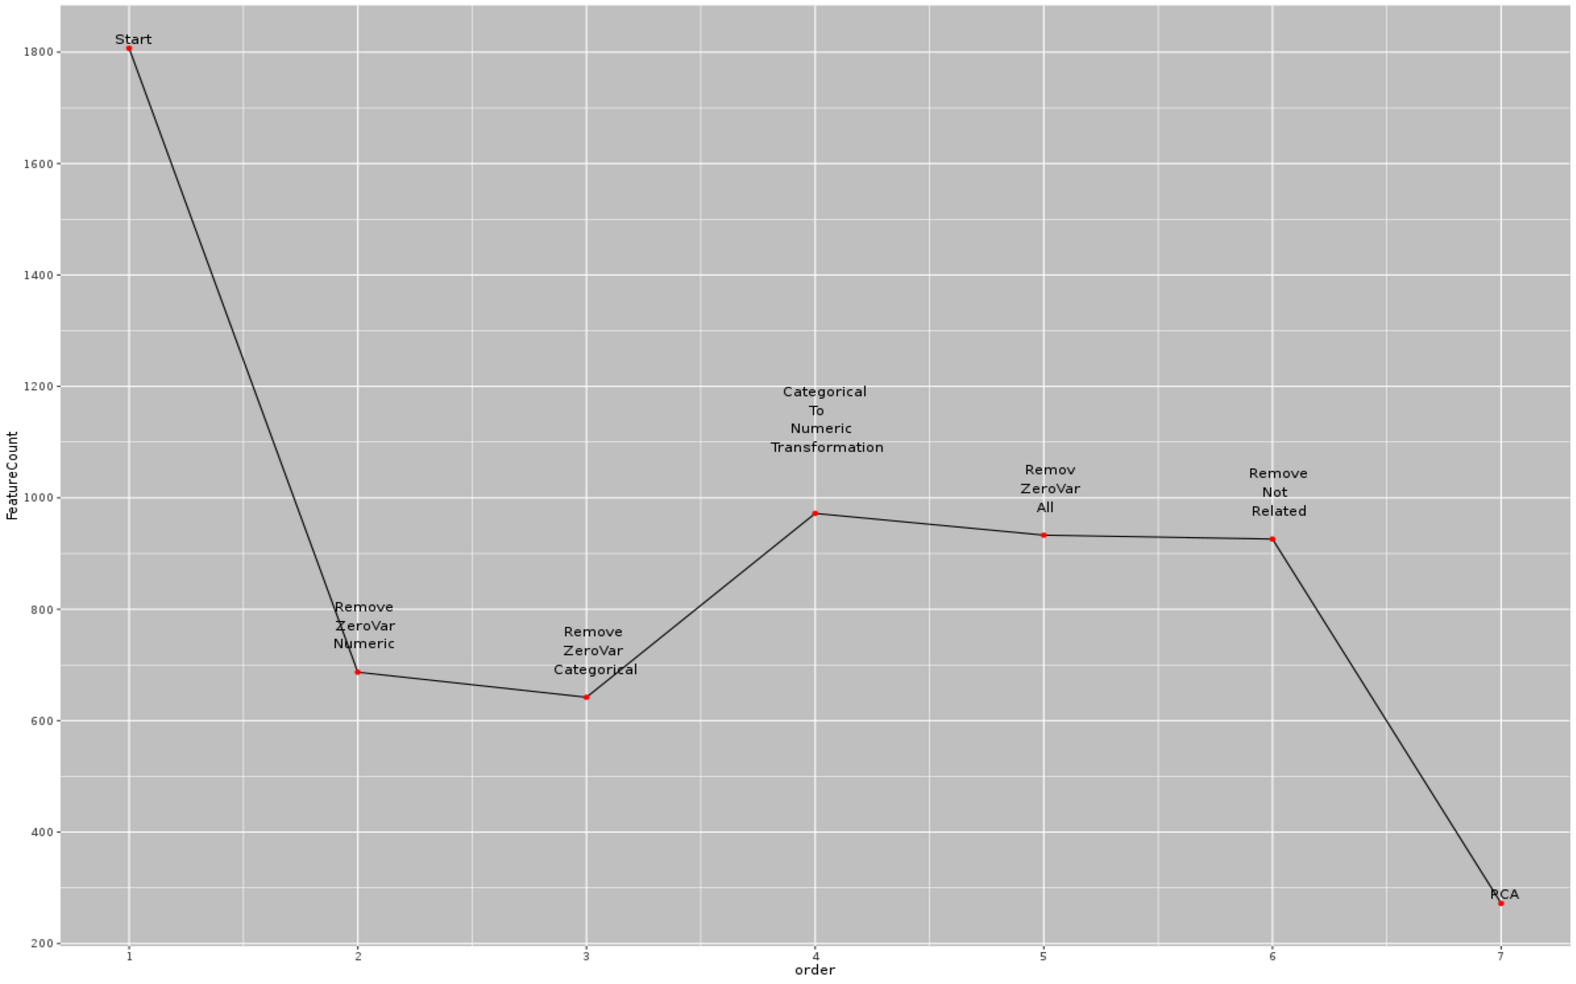
\includegraphics[scale=0.25]{Graphics/preprocessing-features.png}
    \caption{Feature amount changes through preprocessing steps.}
    \label{fig:features-preprocessing}
\end{figure}

\begin{figure}[h!]
    \centering
    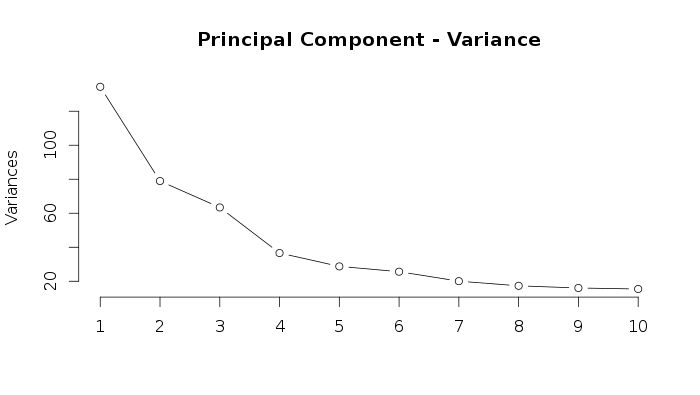
\includegraphics[scale=0.50]{Graphics/PR-Analysis.png}
    \caption{Variance analysis of the particular principal components.}
    \label{fig:pca-var}
\end{figure}

Removing of examples contaminated by data acquisition errors reduced the sample size at \(~1\%\) to \(95.829\) examples.

Overall \(14.594.514\) categorical and \(59.224.282\) numerical feature values are imputed.


\textbf{Machine Learning Results:}

\textbf{One-Class SVM:}




% FAZIIIIIIT!!!!!





